\documentclass[11pt]{article}
\usepackage[utf8]{inputenc}
\usepackage{graphicx}
\graphicspath{ {images/} }
\usepackage{amsmath}

\title{Coursework 1 – Transient Conduction}
\author{Adam Duncan}
\date{\today}

\begin{document}

\maketitle

\section{\emph{Part A: Using lumped capacitance}}
\begin{figure}[h]
    \centering
    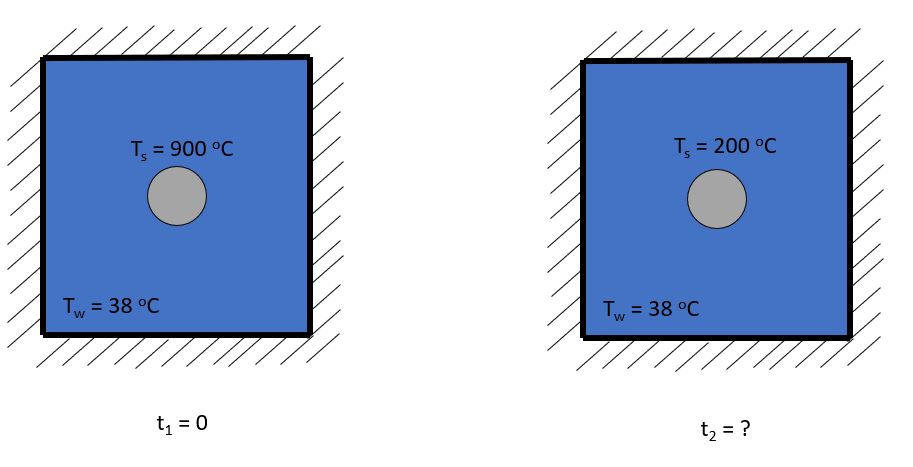
\includegraphics[width=0.85\textwidth]{part_a_fig}
    \caption{Part A schematic at initial and final state.}
    \label{fig:schem_a}
\end{figure}

\begin{equation}
    Bi = \frac{h L_{c}}{k}
\end{equation}
Where $h$ is conductivity [W/mK]

\section{\emph{Part B: Lumped capacitance justification}}
\begin{equation}
t=\frac{f_{0} \rho C_{p} R^{2}}{k}
\end{equation}
\section{\emph{Part C: Transient conduction}}

\section{\emph{Part D: Non-infinite water bath}}

\section{\emph{Part E: Equilibrium temperature}}
\end{document}
